% Para facilitar a manutenção é sempre melhore criar um arquivo por capitulo, para exemplo isso não é necessário

%---------------------------------------------------------------------------------------
\chapter{Descrição da execução do experimento}

	Para a realização deste experimento, foram utilizados o programa Quartus 13.0 SP 1 e a placa \ac{fpga}
Cyclone II - EP2C20F484C7.

	\section{ETAPA 1 – Display de 7 segmentos}
		Para representar um número de 4 \textit{bits} na placa, utilizou-se 4 \textit{switch}, cada um
		representando um bit do número. Como um segmento do \textit{display} pode ser acendido
		em mais de um número,
		motou-se uma expressão lógica para cada segmento do \textit{display}.

		\begin{table}[h]
			\centering
			\caption{Tabela verdade utilizada para chegar na expressão de cada um dos segmentos.}
			\label{table:tabelaVerdade1}
			\begin{tabular}{c|c|c|c|c}
		%\hline
				\textbf{A (SW[4])} & \textbf{B (SW[3])} & \textbf{C (SW[2])} & \textbf{D (SW[1])} & \textbf{Saída em base decimal} \\
				\hline
				0 & 0 & 0 & 0 & 0\\
				0 & 0 & 0 & 1 & 1\\
				0 & 0 & 1 & 0 & 2\\
				0 & 0 & 1 & 1 & 3\\
				0 & 1 & 0 & 0 & 4\\
				0 & 1 & 0 & 1 & 5\\
				0 & 1 & 1 & 0 & 6\\
				0 & 1 & 1 & 1 & 7\\
				1 & 0 & 0 & 0 & 8\\
				1 & 0 & 0 & 1 & 9\\
			\end{tabular}
		\end{table}

		Para o segmento 0 montou-se a expressão
		$$A'.B'.C'.D+A'.B.C'.D'$$
		para o segmento 1 montou-se a expressão
		$$A'.B.C'.D+A'.B.C.D'$$
		para o segmento 2 montou-se a expressão
		$$A'.B'.C.D'$$
		para o segmento 3 montou-se a expressão
		$$A'.B.C'D'+A'.B'.C'.D+A'.B.C.D$$
		para o segmento 4 montou-se a expressão
		$$A'.D+A'.B.C'+B'.C'.D$$
		para o segmento 5 montou-se a expressão
		$$A'.B'.D+A'.C.D+A'.B'.C$$
		para o segmento 6 montou-se a expressão
		$$A'.B'.C'+A'.B.C.D$$.

		Com tais expressões, montou-se o circuito conforme o \autoref{apendice:CircuitoEtapa1}.
		Depois foram realizadas simulações e execução do circuito na placa \ac{fpga}.

	\section{ETAPA 2 – Meio-somador 1 bit}

		A operação aritmética mais simples é a soma de dois dígitos binários. Um circuito combinacional
		que implementa a adição de dois bits é chamado de meio-somador (half adder ou HAD).
		A \autoref{fig:meioSomador} ilustra um esquema de entradas e saída de um meio-somador.
		Um meio-somador de 1 bit deve respeitar a \autoref{table:tabelaMeioSomador}.

		\begin{figure}[H]
			\centering
			\caption{\label{fig:meioSomador}Ilustração de um meio somador.}
			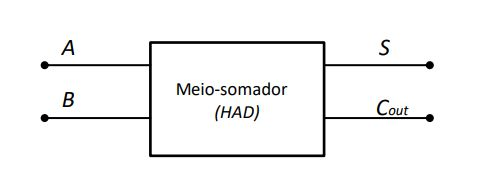
\includegraphics[width=1\textwidth]{img/meioSomador}
		\end{figure}

		\begin{table}[h]
			\centering
			\caption{Tabela verdade de um meio somador.}
			\label{table:tabelaMeioSomador}
			\begin{tabular}{c|c|c|c}
		%\hline
				\textbf{A} & \textbf{B} & \textbf{S (soma)} & \textbf{CarryOut} \\
				\hline
				0 & 0 & 0 & 0\\
				0 & 1 & 1 & 0\\
				1 & 0 & 1 & 0\\
				1 & 1 & 0 & 1\\
			\end{tabular}
		\end{table}

		O circuito deve guardar o \textit{CarryOut} ( o “vai um”) da soma, representando sua existência
		ou ausência através de um LED, ligando-o quando houver o carry, e mantendo-o desligado quando
		o carry não ocorrer.

		A representação esquemática do circuito pode ser encontrada no \autoref{apendice:CircuitoEtapa2}.
	%\section{ETAPA 3 – Meio-somador 4 bits}





%Apresentar   o   detalhamento   da  execução  e   resultados   dos   passos   realizados
%durante   o   experimento,   incluindo   tabelas   verdade,   esquemáticos,   e   código
%(quando  houver).
%Especificar  componentes,  sistemas  e  instrumentos  utilizados.
%Usar listas, figuras e quadros, descrevê-los e discuti-los.



%---------------------------------------------------------------------------------------
